\documentclass[english,,man]{apa6}
\usepackage{lmodern}
\usepackage{amssymb,amsmath}
\usepackage{ifxetex,ifluatex}
\usepackage{fixltx2e} % provides \textsubscript
\ifnum 0\ifxetex 1\fi\ifluatex 1\fi=0 % if pdftex
  \usepackage[T1]{fontenc}
  \usepackage[utf8]{inputenc}
\else % if luatex or xelatex
  \ifxetex
    \usepackage{mathspec}
  \else
    \usepackage{fontspec}
  \fi
  \defaultfontfeatures{Ligatures=TeX,Scale=MatchLowercase}
\fi
% use upquote if available, for straight quotes in verbatim environments
\IfFileExists{upquote.sty}{\usepackage{upquote}}{}
% use microtype if available
\IfFileExists{microtype.sty}{%
\usepackage{microtype}
\UseMicrotypeSet[protrusion]{basicmath} % disable protrusion for tt fonts
}{}
\usepackage{hyperref}
\hypersetup{unicode=true,
            pdftitle={The Unsung Principles of Dynamics},
            pdfauthor={Christopher R. Dishop, Jeffrey Olenick, \& Richard. P DeShon},
            pdfkeywords={\ldots{}.},
            pdfborder={0 0 0},
            breaklinks=true}
\urlstyle{same}  % don't use monospace font for urls
\ifnum 0\ifxetex 1\fi\ifluatex 1\fi=0 % if pdftex
  \usepackage[shorthands=off,main=english]{babel}
\else
  \usepackage{polyglossia}
  \setmainlanguage[]{english}
\fi
\usepackage{graphicx,grffile}
\makeatletter
\def\maxwidth{\ifdim\Gin@nat@width>\linewidth\linewidth\else\Gin@nat@width\fi}
\def\maxheight{\ifdim\Gin@nat@height>\textheight\textheight\else\Gin@nat@height\fi}
\makeatother
% Scale images if necessary, so that they will not overflow the page
% margins by default, and it is still possible to overwrite the defaults
% using explicit options in \includegraphics[width, height, ...]{}
\setkeys{Gin}{width=\maxwidth,height=\maxheight,keepaspectratio}
\IfFileExists{parskip.sty}{%
\usepackage{parskip}
}{% else
\setlength{\parindent}{0pt}
\setlength{\parskip}{6pt plus 2pt minus 1pt}
}
\setlength{\emergencystretch}{3em}  % prevent overfull lines
\providecommand{\tightlist}{%
  \setlength{\itemsep}{0pt}\setlength{\parskip}{0pt}}
\setcounter{secnumdepth}{0}
% Redefines (sub)paragraphs to behave more like sections
\ifx\paragraph\undefined\else
\let\oldparagraph\paragraph
\renewcommand{\paragraph}[1]{\oldparagraph{#1}\mbox{}}
\fi
\ifx\subparagraph\undefined\else
\let\oldsubparagraph\subparagraph
\renewcommand{\subparagraph}[1]{\oldsubparagraph{#1}\mbox{}}
\fi

%%% Use protect on footnotes to avoid problems with footnotes in titles
\let\rmarkdownfootnote\footnote%
\def\footnote{\protect\rmarkdownfootnote}


  \title{The Unsung Principles of Dynamics}
    \author{Christopher R. Dishop\textsuperscript{1}, Jeffrey
Olenick\textsuperscript{1}, \& Richard. P DeShon\textsuperscript{1}}
    \date{}
  
\shorttitle{DYNAMICS PRINCIPLES}
\affiliation{
\vspace{0.5cm}
\textsuperscript{1} Michigan State University}
\keywords{....\newline\indent Word count: 95}
\usepackage{csquotes}
\usepackage{upgreek}
\captionsetup{font=singlespacing,justification=justified}

\usepackage{longtable}
\usepackage{lscape}
\usepackage{multirow}
\usepackage{tabularx}
\usepackage[flushleft]{threeparttable}
\usepackage{threeparttablex}

\newenvironment{lltable}{\begin{landscape}\begin{center}\begin{ThreePartTable}}{\end{ThreePartTable}\end{center}\end{landscape}}

\makeatletter
\newcommand\LastLTentrywidth{1em}
\newlength\longtablewidth
\setlength{\longtablewidth}{1in}
\newcommand{\getlongtablewidth}{\begingroup \ifcsname LT@\roman{LT@tables}\endcsname \global\longtablewidth=0pt \renewcommand{\LT@entry}[2]{\global\advance\longtablewidth by ##2\relax\gdef\LastLTentrywidth{##2}}\@nameuse{LT@\roman{LT@tables}} \fi \endgroup}


\DeclareDelayedFloatFlavor{ThreePartTable}{table}
\DeclareDelayedFloatFlavor{lltable}{table}
\DeclareDelayedFloatFlavor*{longtable}{table}
\makeatletter
\renewcommand{\efloat@iwrite}[1]{\immediate\expandafter\protected@write\csname efloat@post#1\endcsname{}}
\makeatother
\usepackage{lineno}

\linenumbers

\authornote{\ldots{}.

Correspondence concerning this article should be addressed to
Christopher R. Dishop, 316 Physics Rd, Psychology Building Room 348,
East Lansing, MI 48823. E-mail:
\href{mailto:dishopch@msu.edu}{\nolinkurl{dishopch@msu.edu}}}

\abstract{
Begin here\ldots{}


}

\usepackage{amsthm}
\newtheorem{theorem}{Theorem}[section]
\newtheorem{lemma}{Lemma}[section]
\theoremstyle{definition}
\newtheorem{definition}{Definition}[section]
\newtheorem{corollary}{Corollary}[section]
\newtheorem{proposition}{Proposition}[section]
\theoremstyle{definition}
\newtheorem{example}{Example}[section]
\theoremstyle{definition}
\newtheorem{exercise}{Exercise}[section]
\theoremstyle{remark}
\newtheorem*{remark}{Remark}
\newtheorem*{solution}{Solution}
\begin{document}
\maketitle

We -- organizational psychologists -- are increasingly interested in
dynamics and process phenomena. Longitudinal studies are becoming more
prevalent in our literature and the number of time points they employ
appears to be growing. The empirical literature uses the terms
\enquote{dynamics} and \enquote{dynamical} at exponentially larger rates
in recent years (DeShon, 2012). A majority of published methods
literature now focuses on longitudinal data analysis (Aguinis, Pierce,
Bosco, \& Muslin, 2009), and there are a number of great reviews on
dynamic models (Wang, Zhou, \& Zhang, 2016) and issues of time (Beal,
2015; Shipp \& Cole, 2015). Moreover, this interest covers many content
areas, including self-regulation, leadership, and team performance
(Hardy, Day, \& Steele, 2018; Schaubroeck, Lam, \& Peng, 2016).

We have noticed a pattern in how people think about and describe
dynamics in empirical studies. Researchers tend to study and convey
their dynamic process of interest with respect to a statistical model or
class of models. For example, researchers that are familiar with growth
models will talk about the importance of growth in a variable or how
within-person trajectories have been ignored in prior research, they
will then estimate a growth curve, and ultimately convey something about
trends or growth over time and how this has added a new dynamic
perspective to our understanding. \enquote{Growth model thinking,} as
well as other recent ways of discussing how things happen over time,
have produced wonderful insights into important processes in
organizational science, and we see them as initial steps toward
dynamics.

When researchers couch their thinking in a model, however, some concepts
naturally go unnoticed. We are accumulating tremendous knowledge about
our core variables and processes by opening the door of dynamics, but
there are even more principles that have yet to be exposed in our
literature -- we have not yet stepped fully through the door. In this
paper we discuss a variety of dynamics principles; some are concepts
that will reorient how researchers think about dynamics, and others are
statistical properties that, if ignored, could result in biased
inferences.

Below, we first discuss two broad classes of \enquote{thinking with
respect to a statistical model} that have done the hard work -- they are
sets of empirical studies taking initial steps towards dynamics. The
first we refer to as \enquote{growth,} and the second as
\enquote{relationships,} and we discuss example studies in each to
briefly show our field's interest in dynamics and how some researchers
approach it. This first section is not exhaustive, we are simply
sampling a few of the common ways researchers currently think about
dynamics to motivate the core of the paper. There, we will unpack a
variety of dynamics principles that must be incorporated as we enter
this domain.

\hypertarget{stepping-toward-dynamics-growth}{%
\section{Stepping Toward Dynamics --
Growth}\label{stepping-toward-dynamics-growth}}

It is becoming increasingly popular to examine whether something goes up
or down over time -- its trend or growth pattern. Sometimes this idea is
also called \enquote{change.}

Hülsheger (2016) examines fatigue trends. He motivates his study by
stating that his examination of the \enquote{the continuous ebb and flow
of fatigue over the course of the day and about the factors that
influence this temporal ebb and flow} responds to calls to
\enquote{empirically address the dynamic process of recovery and thereby
helps refine recovery theory} (p.~906). For 5 consecutive workdays he
employes fatigue surveys -- one in the morning, another at the first
work break, a third at the end of work, and the last in the evening --
among a sample of Dutch employees. All surveys measure fatigue, and the
morning survey also assessses sleep quality whereas the fourth measures
psychological detachment. He estimates growth curves for fatigue across
his sample and correlates sleep quality and psychological detachment
with both the fatigue intercept and slope, respectively.

Dunford, Shipp, Boss, Angermeier, and Boss (2012) examine burnout
trajectories over two years. They motivate their study by stating that,
\enquote{theoretically, much of the burnout literature suggests that
burnout should be progressive and dynamic, yet most empirical research
has focused on explaining and testing the antecedents of static levels
of burnout,} therefore \enquote{knowing for whom burnout changes and
when this pattern of change occurs leads to a more realistic view of the
dynamism of human experience and better managerial prescriptions for
addressing burnout} (p.~637). Over two years they assess healthcare
workers with five measurements, each separated by six months. All
surveys measure burnout (all dimensions), and the researchers also
collect between person assessments of job transitions (a categorical
variable indicating whether an employee is a newcomer, recently
underwent an internal job change, or remained at the same position
throughout). They estimate a sequence of growth curves and examine
linear and quadratic slope terms for all three burnout dimensions. They
also covary job transition type with the intercept and slope terms.

\hypertarget{summary}{%
\subsection{Summary}\label{summary}}

These authors are clearly interested in dynamics, and in this framework
they examine within-person trajectories, whether those trajectories
exhibit trends (growth), and correlate other variables with those
trends.

\hypertarget{stepping-toward-dynamics-relationships}{%
\section{Stepping Toward Dynamics --
Relationships}\label{stepping-toward-dynamics-relationships}}

Another popular approach is to examine relationships across time rather
than trends or covariates of trend.

Gabriel, Koopman, Rosen, and Johnson (2018) study the association among
helping acts, depletion, and self-serving political acts. They motivate
their study by highlighting the limitations of between-person research
and then stating that \enquote{a more appropriate empirical test of this
process requires an intraindividual lens that allows researchers to
consider how OCBs, resources, and subsequent behaviors vary daily. That
is, not assessing the dynamic relations between helping behaviors and
related constructs potentially misaligns the theoretical underpinnings
of the construct and the level of analysis used to assess their
relationships (i.e., taking dynamic processes and assessing them with
static, \enquote{in general} assessments of constructs; Klein \&
Kozlowski, 2000)} (p.~2). For ten work days they collect surveys twice a
day (morning and afternoon). Both the morning and afternoon surveys
assess helping acts, depletion, and political acts. They regress
afternoon depletion on afternoon helping acts and morning depletion.
They regress afternoon political acts on afternoon depletion and morning
political acts. They regress afternoon helping acts on afternoon
depletion and morning helping acts.

Johnson, Lanaj, and Barnes (2014) study the relationship between justice
behaviors, depletion, and OCBs -- they argue that exhibiting procedural
justice behaviors is depleting and can negatively influence OCBs. They
motivate their study by stating that our current justice knowledge comes
from \enquote{cross-sectional studies examining between-person
differences,} but \enquote{there is a need for longitudinal, daily
investigations of justice experiences that take a dynamic person-centric
view} (p.~1). Ultimately they argue that their research design enabled
them to \enquote{examine dynamic, within-person effects} and test a
model \enquote{via a more granular approach to time} (p.~11). Their
participants responded to surveys twice a day for 10 working days
(morning and afternoon). The morning survey measured sleep quantity,
whereas the afternoon survey measured justice behaviors, depletion, and
OCBs. They regress afternoon depletion on the morning sleep quantity,
the prior day's afternoon justice behavior, and the prior day's
afternoon depletion.

Rosen, Koopman, Gabriel, and Johnson (2016) explore the relationship
between incivility and self-control. They motivate their research by
stating that \enquote{although examinations of incivility have gained
momentum in organizational research, theory and empirical tests
involving dynamic, within-person processes associated with this negative
interpersonal behavior are limited} (p.~1). They also argue that
\enquote{previous studies focused almost exclusively on chronic forms of
incivility that occur on average during unspecified periods of time,
which overlooks the dynamic and temporal nature of incivility and its
effects. Consistent with ego depletion theory, we consider a dynamic
process that explains why employees become more uncivil.} (p.~2). Their
participants respond to three surveys a day (morning, afternoon, and
evening) for 10 workdays. The morning survey assesses self-control, the
afternoon survey assesses self-control, experienced incivlity, and
instigated incivility, and the evening survey measures experienced
incivility and instigated incivility. They regress afternoon
self-control on afternoon incivility and morning self-control. Another
model regresses evening incivility on afternoon self-control.

Koopman, Lanaj, and Scott (2016) examine the costs and benefits of OCBs
on behalf of the actor -- specifically how OCBs relate to positive
affect and work goal progress. They motivate their study by stating that
they \enquote{respond to calls in the literature to examine the
consequences of OCB on a more dynamic basis} (p.~415). Their respondents
fill out three surveys (morning, afternoon, and evening) for ten
workdays. The morning survey assesses OCBs, positive affect, and work
goal progress. The afternoon survey measures work goal progress, and the
evening survey assesses outcome variables irrelevant to the discussion
here. They examine the relationship between OCBs and positive affect by
regressing afternoon positive affect on morning OCB and morning work
goal progress. They examine the relationship between OCBs and work goal
progress by regressing afternoon work goal progress on morning OCB and
morning work goal progress.

\hypertarget{summary-1}{%
\subsection{Summary}\label{summary-1}}

These authors are also interested in dynamics. All test for
within-person variance and motivate their studies by stating that
\enquote{the good stuff} resides in the within-person relationships.
They examine concurrent or lagged relationships across their variables
over time, and they are able to examine many observations due to their
frequent sampling designs.

\hypertarget{dynamics}{%
\section{Dynamics}\label{dynamics}}

Both frameworks above get things moving toward dynamics. They bring up
great notions like within-person trajectories and lag relationships, but
there are many more principles left to appreciate, and we want to expose
our field to them so that researchers have an even greater number of
tools to explore this domain.

Dynamics refers to a specific branch of mathematics/mechanics, but the
term is used in different ways throughout our literature. It is used
informally to mean \enquote{change}, \enquote{fluctuating,}
\enquote{volatile,} \enquote{longitudinal,} or \enquote{over time}
(among others), whereas formal definitions in our literature are
presented within certain contexts. Wang (2016) defines a dynamic
\emph{model} as a \enquote{representation of a system that evolves over
time. In particular it describes how the system evolves from a given
state at time \emph{t} to another state at time \(t + 1\) as governed by
the transition rules and potential external inputs} (p.~242). Vancouver,
Wang, and Li (2018) state that dynamic \emph{variables} \enquote{behave
as if they have memory; that is, their value at any one time depends
somewhat on their previous value} (p.~604). Finally, Monge (1990)
suggests that in dynamic \emph{analyses}, \enquote{it is essential to
know how variables depend upon their own past history} (p.~409).

The crucial notion to take from dynamics, then, is memory. When the past
matters, and future states are constrained by where they were at prior
points in time, dynamics are at play. Below, we unpack a number of
important principles couched in this simple idea.

\hypertarget{concepts}{%
\subsection{Concepts}\label{concepts}}

states vs.~variables memory self-similarity constraints boundary space
on the system reciprocal ando and simon timing. within person dynamics
vs.~entire room temperature

\hypertarget{statistics}{%
\subsection{Statistics}\label{statistics}}

lags equilibrium random walks white noise stationarity

\hypertarget{systems-theory-principles}{%
\section{Systems Theory Principles}\label{systems-theory-principles}}

We start with principles from systems theory -- a gentle place to begin
given that some of the terms will overlap with the growth modeling
literature.

\hypertarget{stocks-and-flows}{%
\subsection{Stocks and Flows}\label{stocks-and-flows}}

One common approach to explaining how things happen over time is to
identify stocks and flows. ({\textbf{???}}) defines both with the
following:

\begin{quote}
A stock is a store, a quantity, an accumulation of material or
information that has built up over time. It may be the water in a
bathtub, a population, the books in a bookstore, the wood in a tree, the
money in a bank, your own self confidence. A stock does not have to be
physical. Your reserve of good will toward others or your supply of hope
that the world can be better are both stocks.
\end{quote}

\begin{quote}
Stocks change over time through the actions of flows. Flows are filling
and draining, births and deaths, purchases and sales, growth and decay,
deposits and withdrawals, successes and failures. A stock, then, is the
present memory of the history of changing flows within the system (18).
\end{quote}

\noindent That last sentence is what makes a stock imply behavior over
time. We speak about stocks by both referring to what they contain right
now but also how they have developed and where they are likely to go.
Also note that stocks do not have to change.

The behavior of a stock -- whether it rises, falls, or remains the same
-- depends on the nature of flows. We can learn about stock behavior by
subtracting outflows from inflows. Doing so leads to three general
principles about stocks. They will ({\textbf{???}}): (1) rise when
inflows exceed outflows, (2) fall when outflows exceed inflows, and (3)
remain the same when inflows equal outflows. In other words, stocks
change with respect to the summative properties of their flows. Stocks
also set the pace for the cumulative rhythm of the system. Even when
flows are changing rapidly, the stock may change slowly because
accumulation occurred over a long period of time.

Figure \ref{stocks} plots a simple stock and flow system over 20 time
periods.

\begin{center}

---------------

Insert Figure \ref{stocks} Here

---------------

\end{center}

\begin{figure}
\centering
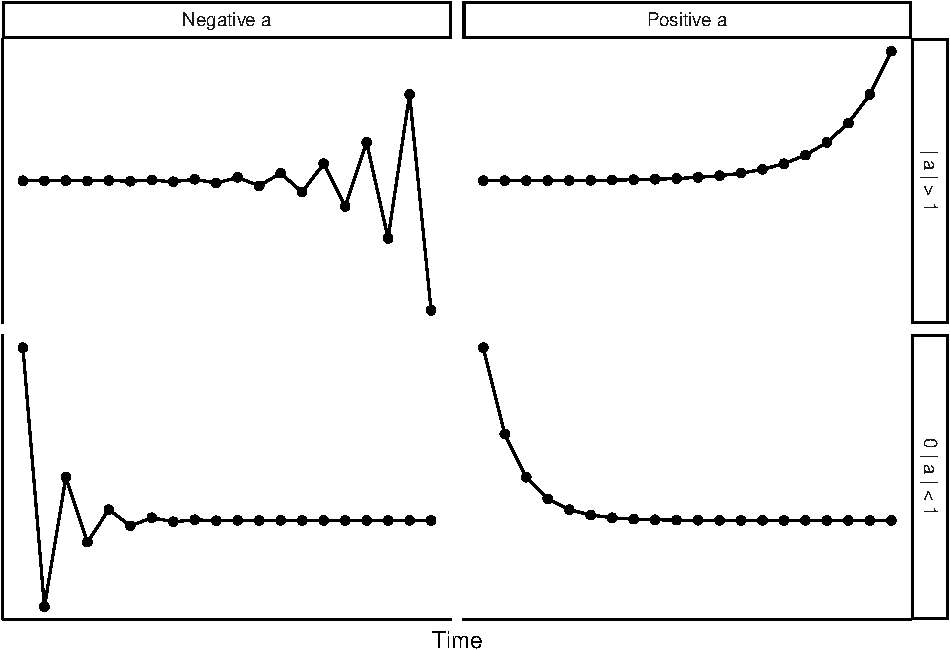
\includegraphics{figs/unnamed-chunk-9-1.pdf}
\caption{\label{fig:unnamed-chunk-9}the ol stock system\label{stocks}}
\end{figure}

\noindent Beginning at the first time point, inflows are equal to
outflows and the stock therefore sits at zero. Over the first ten time
points, however, outflows remain the same whereas inflows increase. With
inflows exceeding outflows the stock also increases up until time point
ten. At this time, inflows drop back down to five whereas outflows
increase -- leading to a large reduction in the stock. As outflows
continue to rise over time -- with no counterbalancing movement from the
inflow -- the stock ultimately decreases.

Systems theory uses stocks and flows as general labels for each of the
things in the system. Above, we described the behavior of the stocks and
flows with simple terms -- increasing, decreasing, or constant. Systems
theory also provides a more systematic way of describing trajectories
and explaining behavior over time. These are unpacked in an excellent
paper by Monge (1990), and the framework includes trend, magnitude, rate
of change, and periodicity. These are shown respectively in figure
\ref{monge}.

\begin{figure}
\centering
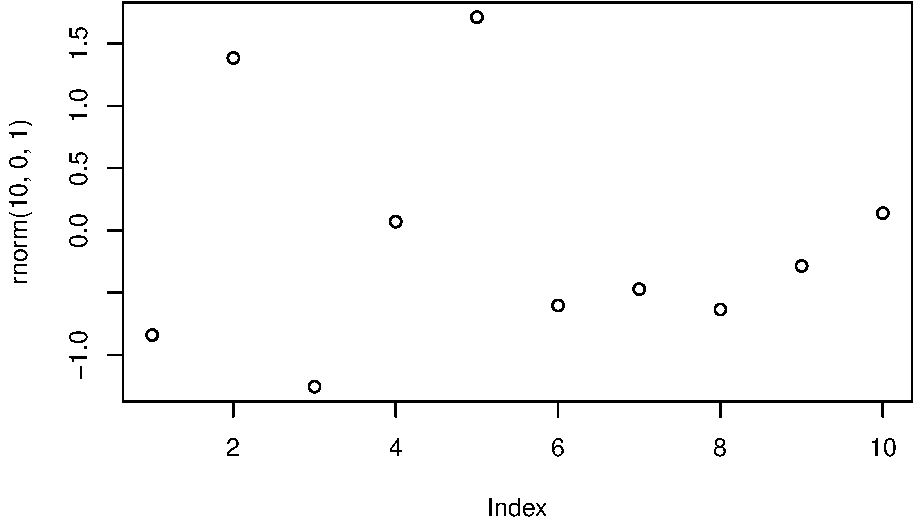
\includegraphics{figs/unnamed-chunk-10-1.pdf}
\caption{\label{fig:unnamed-chunk-10}monge image\label{monge}}
\end{figure}

\begin{center}

---------------

Insert Figure \ref{monge} Here

---------------

\end{center}

\hypertarget{trend}{%
\subsection{Trend}\label{trend}}

Dividing figure \ref{monge} into two portions -- the top and bottom --
reveals differences in trend. All of the panels on the top of the figure
have trend, whereas those on the bottom do not. Trend is the systematic
increase or decrease of a variable over time.

\hypertarget{magnitude}{%
\subsection{Magnitude}\label{magnitude}}

Magnitude is the level, value, or amount of the variable at each time
point -- the number on the \(y\) axis at each respective point in time.
For example, in panel \emph{C} of figure two the magnitude is low at
times 1, 2, and 3, but is high at later points in time. Additionally,
panel \emph{E} and \emph{F} have the same magnitude if we average their
values over time, but panel \emph{E} contains both high and low
magnitude, whereas the magnitude for the trajectory in panel \emph{F}
remains relatively constant.

\hypertarget{rate-of-change}{%
\subsection{Rate of Change}\label{rate-of-change}}

Monge (1990) refers to rate of change as \enquote{How fast the magnitude
increases or decreases per one unit of time.} Panels \emph{G} and
\emph{H} reveal differences in rates of change.

\hypertarget{periodicity}{%
\subsection{Periodicity}\label{periodicity}}

Periodicity is the amount of time before a pattern repeats itself, and
it is equivalent to the term cycle. The most important piece about
periodicity is that it must be couched with \enquote{controlling for
trend.} Notice that panel \emph{A} is periodic because, after
controlling for trend, there are repeated patterns over time.

\hypertarget{two-variables}{%
\subsection{Two Variables}\label{two-variables}}

It is of course possible to combine these notions when researchers are
studying processes with more than one variable. For example, a
researcher might describe the magnitude in their presumed dependent
variable with respect to the magnitude of their independent variable, or
the rates of change across the system of variables. When we turn to the
behavior and relationships among two or more variables -- i.e., a system
of variables -- a few additional principles are available.

\hypertarget{lags}{%
\subsection{Lags}\label{lags}}

How long does it take for the presumed independent variable to produce
an effect on the outcome? This is the notion of lag.

\hypertarget{permanence}{%
\subsection{Permanence}\label{permanence}}

Once the effect happens, how long does it last? That is, if the
independent variable causes the dependent variable to change to a new
value, does the dependent value remain at that new value indefinitely?

\hypertarget{feedback-loops}{%
\subsection{Feedback Loops}\label{feedback-loops}}

Systems theory researchers often convey process by using feedback loops.
Feedback loops describe processes where a variable eventually relates
back to itself.

There are two common ways to describe the behavior of a focal variable
within a feedback loop. When feedback causes the variable to move in the
opposite direction than it initially moved, this is known as negative
feedback, deviation counteraction, or a balancing feedback loop
({\textbf{???}}; Monge, 1990). Here, an initial increase in \(x\) leads
to subsequent changes in the system that, through time, eventually cause
\(x\) to decrease. Now that \(x\) has gone down, more changes happen in
the system that, through time, eventually cause \(x\) to increase.

When feedback, instead, causes the variable to move in the same
direction that it initially moved, this is known as postive feedback,
deviation ampliciation, or a reinforcing feedback loop ({\textbf{???}};
Monge, 1990). Here, changes in \(x\) in one direction lead to eventual
changes in \(x\) in the same direction and thus produce exponential,
explosive, or amplifying behavior. Of course, we can also identify
whether there is positive or negative feedback for every variable in the
system.

\hypertarget{examples}{%
\subsection{Examples}\label{examples}}

People from our literature using these terms and principles to explain
something. Study 1 measured X and Y and described trend. Study 2
measured X and Y and talked about cycles. Study 3 measured X and Y and
reported lags.

\hypertarget{summary-2}{%
\subsection{Summary}\label{summary-2}}

These systems theory notions are valuable tools to explain and describe
process. Note that we did not cover everything to keep the reading
concise and consistent. For example, ({\textbf{???}}) also covers
discontinuous systems, so please refer to his excellent paper for an
even deeper discussion. Now we turn to mathematics and dynamics and
describe principles from these domains that are used to explain or
describe process.

\hypertarget{mathematics-and-dynamics-principles}{%
\section{Mathematics and Dynamics
Principles}\label{mathematics-and-dynamics-principles}}

\hypertarget{difference-equations}{%
\subsection{Difference Equations}\label{difference-equations}}

In mathematics, a basic representation of a process over time is a
difference equation:

\begin{equation}
\label{basicD}
y_{t} = y_{t - 1}
\end{equation}

\noindent where \(y_{t}\) represents \(y\) now and \(y_{t-1}\) is the
variable at the prior time point. Here, the value of \(y\) is the same
at each \(t\), and the emergent behavior would be a flat line across
time. In systems theory terms, there would be no trend.

Although equation \ref{basicD} seems simple, it introduces a fundamental
concept in dynamics: memory. The variable now depends on where it was in
the past. It is constrained, there are boundaries on where it can go.

As we add terms to this basic difference equation the behavior of the
variable becomes more complex. Adding a forcing constant, \emph{c} in
equation \ref{basicD} produces positive or negative trend depending on
whether \emph{c} is, respectively, positive or negative. For example,
the following equation:

\begin{equation}
\begin{split}
\label{diffC}
y_{t} &= y_{t-1} + c \\ 
c &= -4
\end{split}
\end{equation}

\noindent produces a line that decreases by four units at each time
point.

The next level of complexity comes from autoregressive terms, which
represent the extent to which the variable relates to itself over time.
Here,

\begin{equation}
\begin{split}
\label{diffA}
y_{t} &= a y_{t-1} \\ 
a &= 0.5
\end{split}
\end{equation}

\noindent the variable is described over time but it does not retain the
same value at each \(t\). Instead, the variable is \emph{similar} over
time and the autoregressive term, \(a\), describes the extent of that
similarity. In equation \ref{diffA}, \(a\) is 0.5, meaning that the
relationship between the variable now and itself at the next time point
will be 0.5.

There are fundamental behaviors of dynamic variables based on their
autoregressive terms, and these are shown in figure \ref{dynamics_plot}.
The top row of figure \ref{dynamics_plot} shows the trajectory of
variables with autoregressive terms that are greater than one in
absolute value. These large terms produce explosive behavior --
exponential growth when \(a\) is positive and oscillating chaos when
\(a\) is negative. When the autoregressive term falls between zero and
one in absolute value, conversely, the variable converges to equilibrium
-- shown in the bottom two panels. Either the variable oscillates at a
decreasing rate until it reaches equilibrium (when \(a\) is negative) or
it converges there smoothly (when \(a\) is positive).

\begin{figure}
\centering
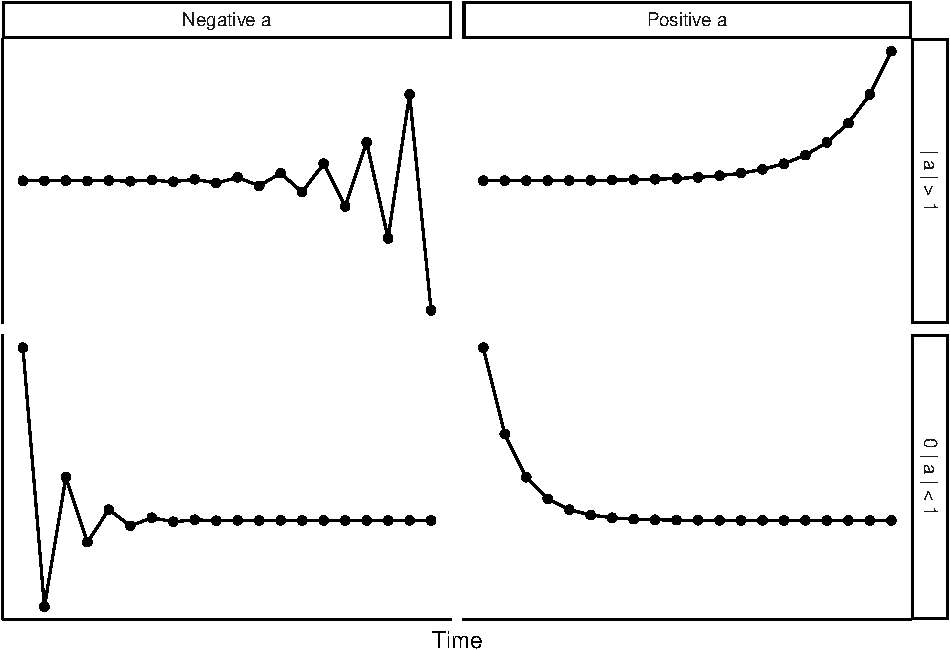
\includegraphics{figs/unnamed-chunk-11-1.pdf}
\caption{\label{fig:unnamed-chunk-11}dynamic equilibrium
fig\label{dynamics_plot}}
\end{figure}

\begin{center}

---------------

Insert Figure \ref{dynamics_plot} Here

---------------

\end{center}

\hypertarget{equilibrium}{%
\subsection{Equilibrium}\label{equilibrium}}

Notice that we introduced a new term in our description above:
equilibrium. Equilibrium describes the state of a variable that no
longer changes unless disturbed by an outside force. It can also be used
to describe multiple variable systems -- where equilibrium again means
that the state remains constant unless disturbed by an outside force,
but here state refers to the the entire system (i.e., all of the
variables). In \emph{static} equalibriums, the system has reached a
point of stability with no change, whereas \emph{dynamic} equilibrium
refers to systems with changes and fluctuations but no net change. That
is, the variables fluctuate across time in periodic ways but the general
state of the system does not diverge so as to change the behavior of the
entire system.

Predator-prey relationships are a typical example of a system in dynamic
equilibrium. For example, consider a predator-prey relationship between
bobcats and rabbits. As the rabbit population increases, the amount of
available food for the bobcats goes up. Over time, this raises the
population of the bobcats as well. Now with a greater bobcat population,
the rabbit population decreases because more are being killed. Over
time, this reduction in food opportunity decreases the bobcat
population. This back and forth oscillating pattern between variables
describes a dynamic equilibrium. The variables change and there may be
random disturbances to the system across time, but the net dynamics of
the system remain stable -- and therefore this situation is still called
\enquote{equilibrium.}

\hypertarget{stochastics}{%
\subsection{Stochastics}\label{stochastics}}

Our route so far has been deterministic -- the mathematical
representations do not contain error. When we want to convey a process
with error we can consider a host of additional principles. Stochastics,
stated simply, refers to processes with error. Consider our simple
difference equation from above, adding an error component produces:

\begin{equation}
\label{diffE}
y_{t} = a y_{t-1} + c + e_{t}
\end{equation}

\noindent where all terms are defined above but \(e_{t}\) represents an
error term that is incorporated into \(y\) at each time point. Errors
cause \(y\) to be higher or lower at specific points in time than we
would have expected given a deterministic process. For example, at time
\(t\) the error might push \(y\) to a higher value, and at \(t+1\) to a
lower value. Errors are therefore said to be random because we cannot
predict their value at any specific \(t\). In aggregation (i.e.,
averaged across time), however, positive errors cancel negative errors,
and large errors are less likely than small errors. Any time we have an
accumulation of random error we get a normal distribution (McElreath,
2016). In stochastic systems, therefore, the errors are said to be
distributed \(N(0, 1)\) -- that is, random and unpredictable at any
specific \(t\) but distributed with certain constraints across time.

It can also be helpful to think about what error is not. Anything that
is systematic, predictable, or common (using those in layman's terms)
cannot be error -- leaving error to be the random \enquote{left overs.}
An aggregation of randomness is a normal distribution.

\hypertarget{white-noise-and-random-walks}{%
\subsection{White Noise and Random
Walks}\label{white-noise-and-random-walks}}

There are two fundamental stochastic processes: white noise and random
walks. White noise is a process that only has error. Setting \emph{c}
and \emph{a} to zero in equation \ref{diffE} produces a white noise
process.

\begin{equation}
\begin{split}
\label{whitenoise}
y_{t} &= a y_{t-1} + c + e_{t} \\
a &= 0 \\
c &= 0
\end{split}
\end{equation}

\noindent Here, all we have is error over time. Panel \enquote{A} of
figure \ref{noise} shows the behavior of a white noise process over
time. Random walks are similar, but \emph{a} is now equal to one.

\begin{equation}
\begin{split}
\label{rw}
y_{t} &= a y_{t-1} + c + e_{t} \\ 
a &= 1 \\ 
c &= 0
\end{split}
\end{equation}

\noindent This representation is also an error process, but there is
self-similarity across time. Panel \enquote{B} of figure \ref{noise}
presents a random walk. Although random walks can sometimes appear to be
moving in a systematic direction, ultimately their behavior is
unpreditable: they could go up or down at any moment.

Random walks and white noise are error processes over time. White noise
processes fluctuate randomly, whereas random walks fluctuate randomly
while retaining some self-similarity through time. These two principles
are the null hypotheses of time-series analysis in econometrics -- where
the first task in a longitudinal study is to demonstrate that you are
investigating something that is not a random walk or white noise.

\begin{figure}
\centering
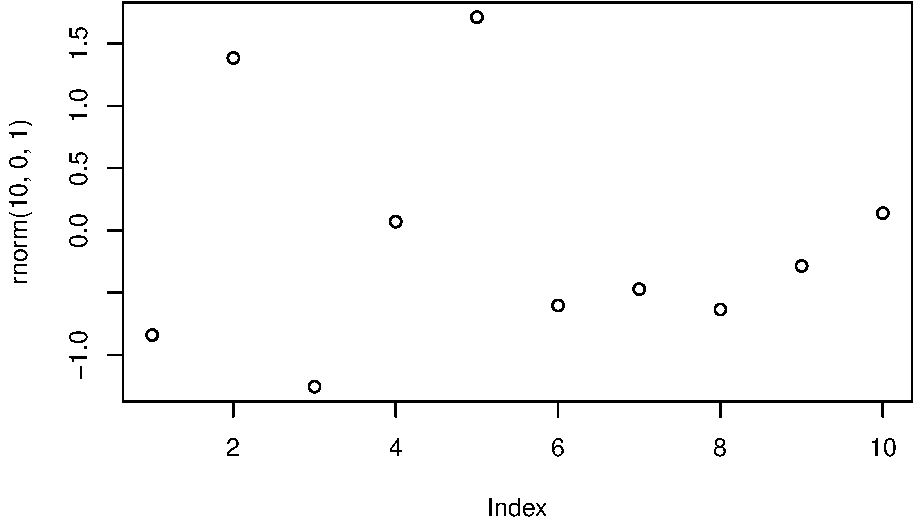
\includegraphics{figs/unnamed-chunk-12-1.pdf}
\caption{\label{fig:unnamed-chunk-12}this one will be a white noise process
and a random walk\label{noise}}
\end{figure}

\hypertarget{system-of-equations}{%
\subsection{System of Equations}\label{system-of-equations}}

Our discussion so far has focused on one variable. Before moving to two
or more variables we want to pause and highlight how much researchers
can explore with single variables. It is of course interesting and fun
to ask how two or more variables are related, or posit a complex
sequence among a set of variables. But understanding whether or not one
variable exhibits white noise or random walk behavior across time is a
valuable study in itself. We feel that our field could substantially
benefit from spending more time plotting and analyzing the individual
trajctories of every measured variable in a study.

With multivariate systems we need multiple equations -- one for each
variable. Before, we demonstrated a simple difference equation for
\(y\). In a multivariate system with two variables, \(x\) and \(y\), we
need one equation for each:

\begin{equation}
\label{sysy}
y_{t} = a y_{t - 1} + e_{t}
\end{equation} \begin{equation}
\label{sysx}
x_{t} = a x_{t - 1} + e_{t}
\end{equation}

\noindent where both equations posit that their variable is a function
of its prior self to the extent of the autoregressive term (\(a\)).
Notice that there are no cross-relationships, we are simply representing
a system with two independent variables across time. It is of course
also possible to introduce relationships among the different variables
with more terms.

First, consider a system where \(x\) concurrently causes \(y\). A more
appropriate way to say this would be that \(x_t\) causes \(y_t\):

\begin{equation}
\label{sysy2}
y_{t} = a y_{t - 1} + b x_{t} + e_{t}
\end{equation} \begin{equation}
\label{sysx2}
x_{t} = a x_{t - 1} + e_{t}
\end{equation}

\noindent where all terms are defined above but now the equation for
\(y\) also includes \(x_{t}\), the value of \(x\) and time \(t\), and
\(b\), the coefficient relating \(x\) to \(y\). This set of equations
says that \(x\) is simply a product of itself over time (with error),
whereas \(y\) is a function of itself and also \(x\) at the immediate
time point.

What if there is a lag between when \(x\) causes \(y\)? That is, perhaps
we posit that \(x\) does not immediately cause \(y\) but instead causes
\(y\) after some period of time. If the lag effect were 2, that would
mean that \(x_t\) causes \(y_{t + 2}\), and to express the \enquote{lag
2 effect} mathematically we would use the following.

\begin{equation}
\label{sysy3}
y_{t} = a y_{t - 1} + b x_{t - 2} + e_{t}
\end{equation} \begin{equation}
\label{sysx3}
x_{t} = a x_{t - 1} + e_{t}
\end{equation}

\noindent Here, all terms are nearly identical to what we saw above but
now there is a lag-two effect from \(x\) to \(y\). \(y\) is now a
function of both its immediately prior self and the value of \(x\) from
two time points ago.

What if we want to convey feedback, or a reciprocal relationship between
\(x\) and \(y\)? That is, now we posit that both \(x\) causes \(y\) and
\(y\) causes \(x\). To do so we update our equations with a simple
change:

\begin{equation}
\label{sysy3}
y_{t} = a y_{t - 1} + b x_{t - 2} + e_{t}
\end{equation} \begin{equation}
\label{sysx3}
x_{t} = a x_{t - 1} + b y_{t - 2} + e_{t}
\end{equation}

\noindent where all terms are defined above but now \(x\) and \(y\) are
reciprocally related. Both are determined by themselves at the
immediately prior time point and the other variable two time points in
the past. \(x\) happens, and two moments later this influences \(y\),
and two moments later this influences \(x\), and so on throughout time.
All the while, both variables retain self-similarity -- they change and
develop but only under the constraints afforded by the autoregressive
terms.

We can make the equations more complicated by continuing to add
variables or longer/shorter lag effects, but the beauty of math is its
freedom to capture whatever the researcher desires. These equations are
language tools to help researchers convey a process over time. If we
were to plug values into the coefficients and variables we would produce
trajectories over time, and to describe those trajectories we could then
use terms like \enquote{trend,} \enquote{periodicity,} or
\enquote{feedback} like we saw in the systems theory section.

\hypertarget{examples-1}{%
\subsection{Examples}\label{examples-1}}

People from our literature using these principles to explain something.
Study 1 argued for random walk behavior in X. Study 2 measured X and Y
and posited an equation.

\hypertarget{summary-3}{%
\subsection{Summary}\label{summary-3}}

\hypertarget{computational-principles}{%
\section{Computational Principles}\label{computational-principles}}

Above, we unpacked representations most people are familiar with: verbal
descriptions, plots, and math. There has recently been a push to use
computational models -- where the goal is still to convey process but in
computer code. In this section we discuss several principles that
researchers can use when they are explaining a process and expect that
explanation to eventually be evaluated with a computational model. We
are not going to show code or a set of scripts or \enquote{if
statements} (although doing so would be a valuable paper on its own).
Instead, the principles below are pieces that should be incoporated into
an explanation if the researcher hopes to eventually evaluate it in a
computer simulation. This section will also be different from the
sections above because we will use a running example throughout, and the
example comes from ({\textbf{???}}).

While developing his notion of satisficing Simon wrote a paper exploring
simple rules that could yield adaptive behavior. His paper was not
framed as a \enquote{computational model,} but his writing is a great
example of how authors can write verbal explanations that lend
themselves to computer simulations. Writing equations is of course
preferred, but the concepts below are tools/criteria for researchers
without a strong mathematical background.

\hypertarget{key-states}{%
\subsection{Key States}\label{key-states}}

Simon's (1956) paper is about how agents move through an environment and
choose among multiple goals -- it is about multiple goal
self-regulation. He begins by arguing that agents choose among multiple
goals to satisfy needs, and need satisfaction is the core driver of
behavior. There are of course other causes, but everything is done with
respect to the need requirements. The two needs he includes are food and
water.

Simon begins his explanation with needs, and although there are other
causes of behavior he makes the assumption that needs are the lowest
level of abstraction required to explain his model. They can be thought
of as the \enquote{foundation} variables to build from. Researchers
should be clear about the core variables that drive all other behavior
in their models. Variables are called \enquote{states} when we talk
about them over time, so the first principle is to adequately identify
and describe the key states.

\hypertarget{state-dynamics}{%
\subsection{State Dynamics}\label{state-dynamics}}

Once we identify the states we need to describe their behavior over
time. Again, Simon's (1956) key states are food and water, and he then
goes on to describe how they unfold as time progresses. He posits that
an agent's food and water states decrease over time because his or her
body requires energy. The body is constantly using food and water in its
stores, so as time passes the key states naturally decrease.

\hypertarget{actions}{%
\subsection{Actions}\label{actions}}

The key states are the assumed \enquote{proximate} causes of behavior,
and we have now explained how they unfold over time. Next, we need to
explain the list of possible behaviors that the causes lead to. In other
words, we need actions that result given the set of states and their
current dynamics. In Simon's model he lists three agent actions:
resting, exploring, and goal striving. These actions satisfy the
internal state dynamics. How so? That is the next criteria.

\hypertarget{action-selection}{%
\subsection{Action Selection}\label{action-selection}}

Assuming a set of actions, how does the agent select among them? Action
selection is the principle for explaining how one of the actions
actually occurs given the states and their dynamics. Simon argues that
if the food and water states are above threshold then the agent rests.
That is, he suggests that the food and water states act like stores
(although they constantly decrease) and only produce action when some
negative discrepancy exists. When one of the states dips below threshold
the agent explores its environment. During exploration the agent
randomly runs into objects, and if he or she encounters a single object
relevant to one of the needs the agent acquires it. If instead the agent
encounters two or more need-relevant objects he or she makes a decision
based on the ratio of effort required to get the object versus the size
of the state discrepancy. In summary, action selection is about how
behavior occurs given the states and their dynamics, whereas actions are
simply the names of the behaviors themselves.

\hypertarget{environment}{%
\subsection{Environment}\label{environment}}

Finally, computer simulations require a structure or environment for
agents to operate within. The environment could be a lattice, a
well-mixed population, or any number of network arrangements, but the
core idea is that context shapes what ultimately happens. Simon explains
his simple rules model within a grid that contains spatially distributed
sources of food and water. The size of the food and water stocks are
determined by the availability of the resources in the environment.
Water is easier to come by than food and so food requirements are
greater.

\hypertarget{summary-4}{%
\subsection{Summary}\label{summary-4}}

\hypertarget{discussion}{%
\section{Discussion}\label{discussion}}

Having presented the principles and terms like process, longitudinal,
and dynamics, we close with our opinion about how the term
\enquote{process} should be used. In our view, only explanations about
the proposed \enquote{true} mechanism should be called
\enquote{process.} If a researcher, instead, simply observes and
describes manifest behavior like trend or correlates of trend then they
are not explaining process -- but it is still a useful study!

\newpage

\hypertarget{references}{%
\section{References}\label{references}}

\setlength{\parindent}{-0.5in}
\setlength{\leftskip}{0.5in}

\hypertarget{refs}{}
\leavevmode\hypertarget{ref-aguinis_first_2009}{}%
Aguinis, H., Pierce, C. A., Bosco, F. A., \& Muslin, I. S. (2009). First
decade of Organizational Research Methods: Trends in design,
measurement, and data-analysis topics. \emph{Organizational Research
Methods}, \emph{12}(1), 69--112.

\leavevmode\hypertarget{ref-beal_esm_2015}{}%
Beal, D. J. (2015). ESM 2.0: State of the art and future potential of
experience sampling methods in organizational research. \emph{Annu. Rev.
Organ. Psychol. Organ. Behav.}, \emph{2}(1), 383--407.

\leavevmode\hypertarget{ref-deshon_multivariate_2012}{}%
DeShon, R. P. (2012). Multivariate dynamics in organizational science.
\emph{The Oxford Handbook of Organizational Psychology}, \emph{1},
117--142.

\leavevmode\hypertarget{ref-dunford_is_2012}{}%
Dunford, B. B., Shipp, A. J., Boss, R. W., Angermeier, I., \& Boss, A.
D. (2012). Is burnout static or dynamic? A career transition perspective
of employee burnout trajectories. \emph{Journal of Applied Psychology},
\emph{97}(3), 637--650.
doi:\href{https://doi.org/http://dx.doi.org.proxy2.cl.msu.edu/10.1037/a0027060}{http://dx.doi.org.proxy2.cl.msu.edu/10.1037/a0027060}

\leavevmode\hypertarget{ref-gabriel_helping_2018}{}%
Gabriel, A. S., Koopman, J., Rosen, C. C., \& Johnson, R. E. (2018).
Helping others or helping oneself? An episodic examination of the
behavioral consequences of helping at work. \emph{Personnel Psychology},
\emph{71}(1), 85--107.

\leavevmode\hypertarget{ref-hardy_interrelationships_2018}{}%
Hardy, J. H., Day, E. A., \& Steele, L. M. (2018). Interrelationships
Among Self-Regulated Learning Processes: Toward a Dynamic Process-Based
Model of Self-Regulated Learning. \emph{Journal of Management},
0149206318780440.
doi:\href{https://doi.org/10.1177/0149206318780440}{10.1177/0149206318780440}

\leavevmode\hypertarget{ref-hulsheger_dawn_2016}{}%
Hülsheger, U. R. (2016). From dawn till dusk: Shedding light on the
recovery process by investigating daily change patterns in fatigue.
\emph{Journal of Applied Psychology}, \emph{101}(6), 905--914.
doi:\href{https://doi.org/http://dx.doi.org.proxy2.cl.msu.edu/10.1037/apl0000104}{http://dx.doi.org.proxy2.cl.msu.edu/10.1037/apl0000104}

\leavevmode\hypertarget{ref-johnson_good_2014}{}%
Johnson, R. E., Lanaj, K., \& Barnes, C. M. (2014). The good and bad of
being fair: Effects of procedural and interpersonal justice behaviors on
regulatory resources. \emph{Journal of Applied Psychology},
\emph{99}(4), 635.

\leavevmode\hypertarget{ref-koopman_integrating_2016}{}%
Koopman, J., Lanaj, K., \& Scott, B. A. (2016). Integrating the Bright
and Dark Sides of OCB: A Daily Investigation of the Benefits and Costs
of Helping Others. \emph{Academy of Management Journal}, \emph{59}(2),
414--435.
doi:\href{https://doi.org/10.5465/amj.2014.0262}{10.5465/amj.2014.0262}

\leavevmode\hypertarget{ref-mcelreath_statistical_2016}{}%
McElreath, R. (2016). \emph{Statistical Rethinking: A Bayesian Course
with Examples in R and Stan} (Vol. 122). CRC Press.

\leavevmode\hypertarget{ref-monge_theoretical_1990}{}%
Monge, P. R. (1990). Theoretical and analytical issues in studying
organizational processes. \emph{Organization Science}, \emph{1}(4),
406--430.

\leavevmode\hypertarget{ref-rosen_who_2016}{}%
Rosen, C. C., Koopman, J., Gabriel, A. S., \& Johnson, R. E. (2016). Who
strikes back? A daily investigation of when and why incivility begets
incivility. \emph{Journal of Applied Psychology}, \emph{101}(11), 1620.

\leavevmode\hypertarget{ref-schaubroeck_can_2016}{}%
Schaubroeck, J. M., Lam, S. S., \& Peng, A. C. (2016). Can peers'
ethical and transformational leadership improve coworkers' service
quality? A latent growth analysis. \emph{Organizational Behavior and
Human Decision Processes}, \emph{133}, 45--58.

\leavevmode\hypertarget{ref-shipp_time_2015}{}%
Shipp, A. J., \& Cole, M. S. (2015). Time in individual-level
organizational studies: What is it, how is it used, and why isn't it
exploited more often? \emph{Annu. Rev. Organ. Psychol. Organ. Behav.},
\emph{2}(1), 237--260.

\leavevmode\hypertarget{ref-vancouver_translating_2018}{}%
Vancouver, J. B., Wang, M., \& Li, X. (2018). Translating Informal
Theories Into Formal Theories: The Case of the Dynamic Computational
Model of the Integrated Model of Work Motivation. \emph{Organizational
Research Methods}, 109442811878030.
doi:\href{https://doi.org/10.1177/1094428118780308}{10.1177/1094428118780308}

\leavevmode\hypertarget{ref-Wang2016}{}%
Wang, M., Zhou, L., \& Zhang, Z. (2016). Dynamic modeling. \emph{Annual
Review of Organizational Psychology and Organizational Behavior},
\emph{3}(1), 241--266.
doi:\href{https://doi.org/10.1146/annurev-orgpsych-041015-062553}{10.1146/annurev-orgpsych-041015-062553}


\end{document}
